% !TeX spellcheck = pl_PL
\newpage\section{Implementacja} \label{sec:implementacja}
Rozdział przedstawia opis wybranych technik użytych do utworzenia głównych funkcji systemu. Techniki te zostały podzielone na cztery kategorie:
\begin{itemize*}
	\item Aplikacja mobilna opisująca implementacje przechowywania danych, graficznych widoków, walidacji danych oraz komunikacji z serwerem. 
	\item Serwer opisujący implementację serwera  oraz strony internetowej wraz z opisem komunikacji między oprogramowaniem serwera a bazą danych.
	\item  Urządzenie sterujące opisujące implementację urządzenia odpowiedzialnego za sterowanie fizyczne dostępem do zamka wraz z komunikacją z serwerem.
	\item Moduł zliczania osób opisujące oprogramowanie odpowiedzialne za zliczanie osób w danym pomieszczeniu. 
\end{itemize*} 
\subsection[Aplikacja mobilna]{Aplikacja mobilna [\StudentB]}
 Aplikacja mobilna jest  modułem odpowiedzialnym za interakcję użytkownika z systemem. Umożliwia on autoryzację, zarządzanie przez administratora systemem oraz uzyskiwanie dostępu do pomieszczenia.
	\subsubsection{Przechowywanie danych}
	W aplikacji mobilnej zostały zaimplementowane 3 możliwości przechowywania danych. Pierwszą z nich jest możliwość trzymania ich w pamięci telefonu jako pliki. Obiekty te przechowywane są w katalogu aplikacji. Przechowują one odpowiednio:
	\begin{itemize*}
	\item	klucz szyfrujący użytkownika zaszyfrowany hasłem użytkownika
	\item certyfikat klucza szyfrującego 
	\item certyfikaty dostępowe
	\end{itemize*}	
	Istnieje możliwość eksportowania dwóch pierwszych plików (Listing: \ref{lst:kod1}) ze względu na brak możliwości ich odzyskania oraz umożliwieni użytkownikowi z korzystania w wielu urządzeniach z tego samego klucza szyfrującego. W przypadku kiedy użytkownik zgubi telefon lub  wyczyści dane aplikacji to wszystkie dane znajdujące się w pamięci telefonu zostaną skasowane. Eksport ten odbywa się w widoku ustawień. Te dwa pliki zostają połączone w jeden plik który zostaje zaszyfrowany hasłem. Plik zapisywany jest w miejscu na telefonie gdzie wskażę użytkownik.  Operacje na pliku wykonywane są przy pomocy klasy statycznej ''FileReadWriteApi''.
	
	Wybór  tej technologi do wymienionych powyższych danych jest uzasadniony zwiększoną trwałością ich w stosunku do danych przechowywanych w pamięci aplikacji jak np.  w klasie globalnej oraz możliwość przechowywania bardziej skomplikowanych danych.
		
	Drugim sposobem przechowywania danych jest funkcja androidowa SharedPreferences. Przechowuje ona proste typy danych takiej jak int, string, char, bool w postaci klucz (wartość typu string) value (wartość z danego typu, który się podało). W pamięci tej przechowuje takie dane jak:
	\begin{itemize*}
		\item adres ip serwera,
		\item login użytkownika,
		\item hasło użytkownika zaszyfrowane kluczem wszytym w oprogramowanie,
		\item token sesji użytkownika,
		\item informacja czy użytkownik aplikacji jest zalogowany,
		\item informacja czy użytkownik aplikacji jest administratorem.	
	\end{itemize*}
\newpage
	\begin{lstlisting}[caption={Funkcja eksportująca klucz szyfrujący.}, label={lst:kod1}, language=Kotlin]
fun exportKey(path:String,password:String){
  if(!Valdiation.isCorrectPassword(password)){
    view.showMessage("niepoprawne haslo")
    view.showErrorPasswordKey()
  }
  try {
    val privateKey = fileReadWriteApi.readFromFile("*" + model.login, view)
    val publicCert = fileReadWriteApi.readFromFile("**" + sharedPreferenceApi.getString(view, EnumChoice.login), view)	
    val str = "{\"public\":" + publicCert + ", \"private\": \"" + privateKey + "\"}"
    val toSend = CyptographyApi.encrypt(str, password)
    fileReadWriteApi.writeToFile(toSend, view, path, true)
    view.showMessage("poprawnie wyeksporotwano certyfikat")
  }
  catch (ex:Exception){
    view.showMessage("Wystapil blad podczas eksportu pliku")
  }
}
	\end{lstlisting}	

	Ponadto przechowuje informacje wykorzystywane w widokach generowania certyfikatu takie jak:
	\begin{itemize*}
		\item wybór loginu,
		\item wybór zamka,
		\item imię, 
		\item nazwisko.
	\end{itemize*}	

	Przykładowy fragment kodu odczytujący dane z SharedPreferences znajduje się na Listingu \ref{lst:kod2}. Dzięki temu rozwiązaniu unikamy ''literówek'', które powodować, by mogły błędy w odczycie danych. 
		
	\begin{lstlisting}[caption={Fragment kodu odpowiedzialny za odczytanie tokenu}, label={lst:kod2}, language=Kotlin]
val token = CyptographyApi.decrypt( sharedPreferenceApi.getString (view, EnumChoice.token))
	\end{lstlisting}
	
	Wybór tej technologi został podyktowany zwiększona trwałością danych w stosunku do klasy globalnej oraz prostotą w użytkowaniu jej. Żeby jeszcze bardziej ułatwić wykorzystywanie tej techniki została napisana specjalna klasa statyczna SharedPreferencesApi, w której został zaimplementowany klasa EnumChoice \linebreak (Listing \ref{lst:kod3}) przechowujący wszystkie klucze.
	
		\begin{lstlisting}[caption={klasa EnumChoice.}, label={lst:kod3}, language=Kotlin]
enum class EnumChoice(val value:String){
  ip("ipserwer"),
  password("password"),
  token("sessionToken"),
  login("login"), 
  nameuser("name"), 
  surname("surname"),
  isLogin("isLogin"), 
  isAdmin("isadmin"),
  choiceLogin("choiceLogin"), 
  choiceLock("choiceLock"),
  publicKey("publicKey")
}
		\end{lstlisting}
		
	Trzecim sposobem jest przechowywanie w klasie globalnej (GlobalContainer)  obiektów. Przechowywane w niej są wszystkie dane które nie wymagają przechowywania po wyłączeniu aplikacji.
		
	\subsubsection{Implementacja graficzna}
		
	Wszystkie wartości typu string wyświetlane na ekranie są przechowywane w pliku Strings znajdującego się w katalogu res/values. Wybór takiego sposobu został podyktowany faktem możliwości późniejszego łatwiejszego przerabiania tekstów oraz możliwości łatwiejszego tłumaczenia na inny język. Wszystkie kolory użyte w aplikacji przechowywane są w pliku colors. Ma to na celu ułatwienie  zmiany kolorów w całej aplikacji. Styl dla podstawowych elementów graficznych takich jak ''editText'', ''TextView'' czy ''Button'' przechowywane są w pliku styles co ma za zadanie umożliwienie łatwiejszej zmiany wyglądów danych elementów w całej aplikacji.
		
	Oprócz stylów elementów, czy wartości tekstowych należy również napisać, w jaki sposób generowane są widoki. Widoki te są przechowywane w plikach XML.  Dla widoków które nie posiadały listy został zaimplementowany układ ''LinearLayout'' ze względu na prostotę w tworzeniu oraz ewentualnych zmianach w wyglądzie. Natomiast dla widoków z wyświetlanymi jakimiś listami został zaimplementowany układ ''ConstrainLayout'' ze względu na fakt że przy liście występuje znacznie więcej odwołań do generowania widoku a układ ten jest pod tym względem o wiele wydajniejszy od wspomnianego wcześniej ''LinearLayout''\cite{desingMobile}.

	\subsubsection{Walidacja danych wprowadzanych przez użytkownika}
	Walidacja danych wprowadzonych przez użytkownika odbywa Się przy pomocy klasy statycznej Validation. Klasa ta udostępnia cztery funkcje odpowiedzialne za:
	\begin{itemize*}
	\item poprawność formatu adresu ip ,
	\item czy data podana w drugim parametrze jest datą późniejszą niż data podana w pierwszym parametrze (Listing \ref{lst:kod5}),
	\item poprawność hasła,
	\item poprawność loginu.
	\end{itemize*}

	Wyrażenia regularne użyte w tych funkcjach znajdują się na Listingu \ref{lst:kod4}.
	
	\begin{lstlisting}[caption={Wyrażenia regularne.}, label={lst:kod4}, language=Kotlin]
  "^(?=.*[0-9])(?=.*[A-Z])(?=.*[@#$%^&+=!])(?=\\S+$).{4,}$"
 
  "^((0|1\\d?\\d?|2[0-4]?\\d?|25[0-5]?|[3-9]\\d?)\\.)
  {3}(0|1\\d?\\d?|2[0-4]?\\d?|25[0-5]?|[3-9]\\d?)$"
		\end{lstlisting}

	\begin{lstlisting}[caption={Funkcja odpowiedzialna za sprawdzanie, która data jest pó"zniejsza.}, label={lst:kod5}, language=Java]
public static boolean biggerThanTime(String time1,String time2){
  Date date = new Date() ;
  SimpleDateFormat dateFormat = new 
  SimpleDateFormat("HH:mm") ;
  dateFormat.format(date);
  try 
  {
    if (dateFormat.parse(time1).after( dateFormat.parse(time2))) {
      return false;
    } else {
      return true;
    }
  }
  catch (Exception ex){}	
  return false;
}
	\end{lstlisting}

	\subsubsection{Komunikacja z serwerem}
	Do komunikacji z serwerem napisana została specjalna klasa dziedzicząca po klasie AsyncTask o nazwie HTTPRequest. Klasa ta wysyła podane w konstruktorze (listing \ref{lst:kod6}) w postaci Hashmap-u dane do serwera i po otrzymaniu informacji zwrotnej z serwera przekazuje tą odpowiedź. Odpowiedź ta jest przekazywana do klasy która utworzyła i wykonała klasę HTTPRequests do funkcji o nazwie podanej w parametrze konstruktora przy pomocy refleksji (listing: \ref{lst:kod7}). Dzięki temu klasa ta jest uniwersalna i Może być stosowana w każdym miejscu programu.
	
	\begin{lstlisting}[caption={Konstruktor klasy HTTPRequest.}, label={lst:kod6}, language=Java]
public HTTPRequestAPI(Object presenter,String url,String methodName,HashMap DataToSend) {
  this.urlString=url;
  this.DataToSend=DataToSend;
  this.methodName=methodName;
  this.presenter=presenter;
}
\end{lstlisting}	
	
\begin{lstlisting}[caption={Metoda OnPost zwracająca odpowied"z serwera.}, label={lst:kod7}, language=Java]
@Override
protected void onPostExecute(String response) {
java.lang.reflect.Method method;
try {
  method = presenter.getClass().getMethod(methodName, String.class);
  method.invoke(presenter, response);
  }
  catch(Exception ex){}
}
\end{lstlisting}	

\subsection{Serwer}
Serwer systemu zarządza wszystkimi informacjami, jest pośrednikiem w przekazywaniu i modyfikacji rekordów z bazy danych MySQL. Emulowaniem środowiska MySQL oraz Apache zajmuje się program XAMP w wersji 3.2.2.
 
	\subsubsection{Aplikacja serwerowa [\StudentA]}\label{sec:apk serw}
	Aplikacja serwerowa została zaimplementowana przy użyciu języka programowania Python 2.7 oraz frameworku Django. Program  właściwie składa się głównie z 3 plików:
	\begin{itemize*}
		\item setting.py --- odpowiedzialny za konfigurację połączenia z bazą danych, zwracanymi komunikatami, kodowanie, strefą czasową i innymi parametrami o mniejszym znaczeniu,
		\item urls.py --- przechowywana tu tablica obiektów URL ustala, dla jakiego adresu URL (pierwszy parametr), wykonać konkretną metodę (parametr view), listing \ref{lst:python url} przedstawia fragment pliku urls.py,
		\item views.py --- główny skrypt serwera, zawiera główną logikę aplikacji, to znaczy metody wykonywane dla konkretnych adresów URL.
	\end{itemize*}

{\footnotesize 
\begin{lstlisting}[caption={Fragment pliku urls.py}, label={lst:python url}, language=Python]
urlpatterns = [
  url(r'^$', views.website, name='home'),
  url(r'^login/$', auth_views.login, {'template_name': 'login.html'}, name='login'),
  url(r'^logout/$', auth_views.logout, {'template_name': 'logged_out.html'}, name='logout'),
  url(r'^list/$', views.website, name='list'),
  url(r'^api/login/$', views.api_login, name='api_login'),
  ...
]
\end{lstlisting}}

	Funkcjonalności systemu w  dużej mierze wymagają stanu zalogowania, weryfikowane jest to przez podanie od użytkownika loginu oraz tokenu sesji logowania. Pola uzyskane w zapytaniu Http w metodzie POST są porównywane z znajdującymi się w bazie danych. Przykładowe API wymagające weryfikacji logowania znajduje się w listingu \ref{lst:serwer weryfikacja}. Użytkownik wysyła pole ''login'' oraz ''token'', następnie wykonane zostaje zapytanie do bazy danych o aktualnie znajdującą się wartość w rekordzie. Jeżeli wartości się pokrywają i nie są puste, może zostać wykonane polecenie, które chciał wywołać użytkownik. Dodatkowo, gdy operacja wymaga uprawnień administratora, weryfikowana jest flaga w bazie danych, czy dany użytkownik jest administratorem (IS\_ADMIN). Wiersze try except służą nie tylko do zamaskowania błędów działania aplikacji, ale również do zabezpieczenia programu przed podatnością SQL Injection (eliminacja tak zwanego feed backu o błędach przy próbie podawania innych wartości niż zaplanowano w systemie).
	
	Operacje logowania i rejestracji są podstawowymi działaniami, dzięki którym będzie można wykonywać bardziej złożone działania oraz niezbędne do poprawnego funkcjonowania PKI. Listing \ref{lst:serwer login} i listing \ref{lst:serwer register} przedstawiają kompletne funkcje logowania i rejestracji użytkowników. 

	{\footnotesize 
	\begin{lstlisting}[caption={Przykładowe API weryfikujące stan logowania}, label={lst:serwer weryfikacja}, language=Python]
def api_download_all_locks(request):
  if request.method == 'POST':
    login = request.POST.get('login')
    token = request.POST.get('token')
    try:
      cursor = db.cursor()
      cursor.execute("SELECT TOKEN FROM USERS WHERE login='%s'" % login)
      token_from_DB = cursor.fetchone()[0]
      if (token_from_DB == token and token != None):
        ...
    except Exception:
      return JsonResponse({"status": "Invalid"})
	\end{lstlisting}}

	Logowanie wymaga podania loginu w polu 'username' oraz skrótu SHA-256 hasła użytkownika. W pierwszej kolejności (linia 5 do 9) tworzony jest ciąg pseudolosowy, który będzie użyty jako token sesji logowania. Zastosowany generator jest wbudowany w bibliotekę RSA, w tym wypadku tworzone ciągi są kluczem publicznym algorytmu RSA. Następnym krokiem jest pobranie skrótu hasła oraz flag (czy jest administratorem, status konta) z bazy danych. Wiersz 15 decyduje, czy konto użytkownika jest aktywne, jeśli nie, to w linii 24 sprawdzane jest, czy konto zostało aktywowane, jeśli tak, oznacza to, że dane konto zostało zablokowane. W przypadku jednak, gdy konto ma status aktywny, następuje aktualizacja wartości tokenu w bazie danych oraz weryfikacja uprawnień użytkownika. Zwrócony status logowania jako root oznacza, zalogowanie się jako administrator.
	
	Operacja rejestracji wymaga podania unikalnego dla systemu loginu, hasła w postaci skrótu SHA-256, imienia, nazwiska użytkownika oraz wygenerowany klucz publiczny RSA. Pierwszym etapem rejestracji jest weryfikacja, czy podany login znajduje się obecnie w bazie danych użytkowników. W tym celu wykonywane jest zapytanie SQL z filtrem podanego loginu, w przypadku, gdy polecenie zwróci pustą wartość (w języku Python None), oznacza to brak istnienia danego użytkownika w bazie. W przeciwnym wypadku, otrzymania wartości z zapytania, zostaje zwrócona przez serwer odpowiedź błędu loginu (ERROR~LOGIN).
	
	Wiersze 15 do 22 skryptu \ref{lst:serwer register} tworzą certyfikat szyfrujący. Pierwszych 5 linii generuje pseudolosową wartość (wg algorytmu RSA dla klucza publicznego), będącą unikalnym identyfikatorem dla certyfikatu szyfrującego. Następnie dodawany do bazy danych jest użytkownik wraz z utworzonym certyfikatem z polami odpowiednio Public\_Key (przesłany klucz publiczny od użytkownika), Serial\_number (wygenerowana wartość pseudolosowa) oraz Validity\_period (obecna data przedłużona o rok), pozostałe wartości są domyślne (klucz szyfrujący RSA, funkcja skrótu SHA-256 i wersja certyfikatu 1).

	Wiersze od 23 do końca funkcji pobierana jest kompletna zawartość certyfikatu (w formacie JSON), która następnie przesyłana jest, jako odpowiedź zwrotna dla użytkownika. W przypadku błędu konwersji rekordu z bazy danych na format JSON lub błędu bazy danych zwrócona zostanie informacja o błędnym wykonaniu polecenia (status invalid w sytuacji braku dodania certyfikatu do bazy danych lub status ERROR, gdy pojawi się nieokreślony błąd podczas wykonywania procesu rejestracji)\cite{programowanie_aplikacji_webowych}.
	\newpage
	
{\footnotesize
\begin{lstlisting}[caption={API rejestracji}, label={lst:serwer register}, language=Python]	
def api_register(request):
  if request.method == 'POST':
    login = request.POST.get('login')
    password = request.POST.get('password')
    name = request.POST.get('name')
    surname = request.POST.get('surname')
    publickkey = request.POST.get('publickkey')
    
    cursor = db.cursor()
    cursor.execute("SELECT LOGIN FROM USERS WHERE LOGIN='%s'" % login)
    data = cursor.fetchone()
    
    if data is not None:
      return JsonResponse({"status": "ERROR LOGIN"})
    else:
      try:
        random_generator = Random.new().read
        key = RSA.generate(1024, random_generator).publickey().exportKey()
        serial = ""
        for x in key.split("\n")[1:-1]:
          serial += x
        record = [login, password, name, surname, '0', publickkey, '1', serial, datetime.now().replace(year=datetime.now().year + 1)]
        cursor.execute( 'INSERT INTO USERS (LOGIN,PASSWORD,NAME,SURNAME,IS_ADMIN,PUBLIC_KEY, ISACTIVATED, Serial_number, Validitiy_period) VALUES(%s,%s,%s,%s,%s,%s,%s,%s,%s)', record)
        db.commit()
        cursor.execute( "SELECT CONCAT(NAME, ' ', SURNAME) as User_Name, LOGIN as Issuer_name,  PUBLIC_KEY, Serial_number, Validitiy_period, Version, Signature_Algorithm_Identifier, Hash_Algorithm FROM `users` WHERE `LOGIN` = '%s'" % (login))
        db.commit()
        dict_certificate = [dict((cursor.description[i][0], value) for i, value in enumerate(row)) for row in cursor.fetchall()]
        if len(dict_certificate) == 0:
          return JsonResponse({"status": "invalid"})
        else:
          return JsonResponse({"status": "ok", "data": dict_certificate})
      except Exception:
        db.rollback()
        return JsonResponse({"status": "ERROR"})
\end{lstlisting}}
\newpage
{\footnotesize 
	\begin{lstlisting}[caption={API logowania}, label={lst:serwer login}, language=Python]	
	def api_login(request):
	if request.method == 'POST':
	username = request.POST.get('username')
	password = request.POST.get('password')
	
	random_generator = Random.new().read
	key = RSA.generate(1024, random_generator).publickey().exportKey()
	token = ""
	for x in key.split("\n")[1:-1]:
	token += x
	
	try:
	cursor = db.cursor()
	cursor.execute("SELECT PASSWORD, IS_ADMIN, ISACTIVATED FROM USERS WHERE login='%s'" % username)
	data = cursor.fetchone()
	if data[2] == 0:
	if data[0] == password:
	cursor.execute("UPDATE USERS SET TOKEN = '%s' WHERE LOGIN = '%s'" % (token, username))
	db.commit()
	if data[1] == 1:
	return JsonResponse({"status": "root", "token": token})
	else:
	return JsonResponse({"status": "ok", "token": token})
	else:
	return JsonResponse({"status": "ERROR PASSWORD", "token": "invalid"})
	elif data[2] == 1:
	return JsonResponse({"status": "not activated", "token": "invalid"})
	else:
	return JsonResponse({"status": "blocked", "token": "invalid"})
	except Exception:
	return JsonResponse({"status": "ERROR", "token": "Invalid"})
	\end{lstlisting}}

	\subsubsection{Strona internetowa [\StudentB]}
	Strona internetowa została dopisana do projektu serwera w oparciu o framework Django. Zaimplementowane są trzy widoki. Widok logowania, widok wyświetlający historię oraz widok do którego przechodzi się po wylogowaniu. Główny widok możliwy jest do wyświetlenia tylko po zalogowaniu. Login oraz hasło używane do zalogowania należy wygenerować podczas konfiguracji serwera przy pomocy polecenia ''python manage.py createsuperuser'' lub modyfikując wpis w bazie danych ręcznie. Strona internetowa znajduje się w plikach:
	\begin{itemize*}
		\item views.py
		\item urls.py
		\item *.html
	\end{itemize*}
 
	W pliku ''urls.py''(Listing: \ref{lst:python url}) znajdują się adresy URL które korzystają z wbudowanej funkcji django ''auth\_views.login'' służącej do logowania oraz ''auth\_views.logout'' służąca do wylogowania. Plik ''views.py'' posiada API (Listing: \ref{lst:serwer login strona}) wykorzystywane w stronie głównej które pobiera z bazy danych. W plikach z rozszerzeniem html znajduje się implementacja wyglądu strony.
	
	{\footnotesize 
		\begin{lstlisting}[caption={API logowania do strony internetowej}, label={lst:serwer login strona}, language=Python]	
@login_required(login_url="login/")
def website(request):
  try:
    cursor = db.cursor()
    cursor.execute("SELECT DATE, ACCESS, locks_keys.NAME, locks_keys.SURNAME, locks.NAME AS 'ZAMEK' FROM access_to_locks, locks_keys, locks WHERE locks_keys.ID_KEY = access_to_locks.ID_KEY AND locks.ID_LOCK = access_to_locks.ID_KEY ORDER BY DATE DESC")
    rows = cursor.fetchall()
  finally:
    return render_to_response('home.html', {"rows": rows})
		\end{lstlisting}}
\subsection{Urządzenie sterujące [\StudentA]}
Program urządzenia sterującego nasłuchuje połączeń bluetooth (jest serwerem) od urządzeń mobilnych. Aplikacje korzystają z bezpiecznego trybu komunikacji, to znaczy posiadają wbudowany klucz, który musi być po obu stronach połączenia identyczny. Fragment kodu odpowiedzialny za utworzenie bezpiecznego serwera znajduje się w Listingu \ref{lst:RPI bt}. Wiersz związany z kluczem aplikacji znajduje się w linii 5, w linii 6 zostaje przypisany do usług serwera. Każde nawiązanie połączenie z urządzeniem sterującym zostaje odnotowane w pliku log, tak samo jest z odebranymi danymi oraz decyzją przyznania dostępu. 
{\footnotesize 
\begin{lstlisting}[caption={Tworzenie serwera bluetooth}, label={lst:RPI bt}, language=Python]
server_sock = BluetoothSocket(RFCOMM)
server_sock.bind(("", PORT_ANY))
server_sock.listen(1)
port = server_sock.getsockname()[1]
uuid = "fa87c0d0-afac-11de-8a39-0800200c9a66"
advertise_service(server_sock, "BluetoothChatSecure", service_id=uuid, service_classes=[uuid, SERIAL_PORT_CLASS], profiles=[SERIAL_PORT_PROFILE])
\end{lstlisting}}
Istotną rolą urządzenia sterującego jest weryfikacja poprawności certyfikatów. Sprawdzając klucze dostępowe ważne jest potwierdzenie, czy dany klucz ma przyznane uprawniania w konkretnym przedziale czasowym, odpowiedzialna za to jest funkcja ''Check\_access'' znajdująca się w Listingu \ref{lst:RPI check access}. Objaśnienie umieszczonego kodu:
\begin{itemize*}
	\item wiersz 2 --- weryfikacja, czy certyfikat jest aktualny (''None'' oznacza stan aktywny),
	\item wiersz 3 --- sprawdzenie ważności certyfikatu, czy obecna data mieści się pomiędzy datą od której jest ważny certyfikat (date\_from) oraz datą do której jest ważny (date\_to),
	\item  wiersz 4 --- sprawdza specjalną flagę ważnego certyfikatu, czy posiadany jest dostęp stały, bez ograniczania godzin w poszczególnych dniach,
	\item wiersze 6 do 21 --- analiza godzin, w których certyfikat ma dostęp, gdy nie jest ustawiona flaga dostępu stałego,
	\item w każdym niespełnionym wyżej opisanym przypadku zostanie odrzucony dostęp.
\end{itemize*}

{\footnotesize 
	\begin{lstlisting}[caption={Funkcja Check-access urządzenia sterującego}, label={lst:RPI check access}, language=Python]
def Check_access(certificate):
  if certificate.isactual is None:
    if datetime.strptime(certificate.date_from, '%Y-%m-%dT%H:%M:%S') < datetime.now() < datetime.strptime( certificate.date_to, '%Y-%m-%dT%H:%M:%S'):
      if certificate.ispernament == 1:
        return True
      else:
        try:
          day_access = certificate.access_table[date.today().weekday()].split(";")
        except Exception:
          day_access = []
        now = datetime.now()
        if len(day_access) > 0:
          for x in day_access:
            x = x.split("-")
            try:
              x0 = x[0].split(":")
              x1 = x[1].split(":")
              if datetime.now().replace(hour=int(x0[0]), minute=int(x0[1])) <= now < datetime.now().replace(hour=int(x1[0]), minute=int(x1[1])):
                return True
            except Exception:
              continue
  return False
	\end{lstlisting}}
\newpage
\subsection{Moduł zliczania osób [\StudentA]}
	Moduł zliczania osób zaimplementowany jest w zintegrowaniu z urządzeniem sterującym. Głównym problemem zastosowania biblioteki Open-CV w Raspberry Pi jest brak posiadania przez mikrokomputer karty graficznej. Operacje przetwarzania obrazu wydajnie pracują, gdy wykonywane są z wysokim współczynnikiem współbieżności. Brak procesorów graficznych skutkuje przeniesieniem złożonych obliczeń na zwykłe procesory CPU, skutkując nie wydajną pracą (obraz bardzo często się zacina). 
	
	Podczas zwykłej pracy moduł zliczania osób nie posiada interfejsu graficznego, przedstawiony widok na Rys. \ref{rys:Zliczanie osob} został utworzony tylko do celów demonstracyjnych. Zielony prostokąt i czerwona kropka oznaczają wykrytą osobą i jego centralny punkt. Dwie linie, niebieska oznacza granicę, gdzie zliczona osoba ''wychodzi'', a czerwona, kiedy ''wchodzi'', przy czym zawsze jest brana pod uwagę linia druga (ze względu na potrzebę czasu reakcji wykrywania osoby).
	
	\begin{figure}[ht!]
		\centering
		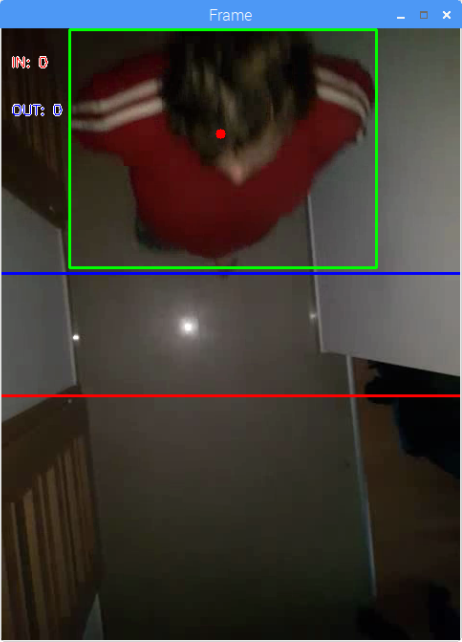
\includegraphics[width=8cm]{Obrazy/Kamera1}
		\caption{Stan początkowy testu zliczania osób (urządzenie sterujące)}
		\label{rys:Zliczanie osob}
	\end{figure}
	
	Algorytm zliczania osób polega na ''śledzeniu'' osób, wykorzystano do tego celu metodę \textit{findContours}. Wcześniej, aby przygotować obraz należy wykonać binarną różnicę obrazu pierwszego (zarejestrowanego bez żadnej osoby w obiektywie) z obrazem obecnym, służy do tego funkcja \textit{threshold}. 
	
	Posiadając listę wykrytych obiektów (poruszających się) następuje filtracja obiektów zbyt małych (możliwych błędów wykrycia ruchu). Kolejnym krokiem jest sprawdzenie, czy istnieje ''osoba'', znajdująca się w obszarze wiążącym ją z wykrytym obiektem, jeśli tak, następuje aktualizacja współrzędnych danej osoby, w przeciwnym wypadku ''pojawia'' się nowa osoba. Rozpoznanie, czy dana osoba wchodzi, czy wychodzi z pomieszczenia polega na prześledzeniu ścieżki jaką przebyła. W zależności od ustawień, osoba idąca ''w górę'' będzie liczona, jako wejście, a ''w dół'' jako wyjście. Istnieje możliwość błędnego odczytu osoby, dlatego w przypadku, gdy osoba nie przemieści się przez 5 odczytów z kamery, zostaje usunięta z listy weryfikowanych \cite{rozpoznawanie_twarzy}.